\chapter{}\label{ex:aufg6}
%
\section{}\label{sec:aufg6a}
%
Da die Kennlinie aus Abb. \ref{dia:uf_kennlinie} sich auf den Scheitelwert der Strangspannung bezieht, wir aber den Effektivwert der Außenleiterspannung benötigen, muss dieser noch durch $\sqrt 2$ geteilt und mit $\sqrt 3$ multipliziert werden.
Als Faktor wird die Steigung der Kennlinie verwendet
\begin{equation}
	U_{\text{max}} = \frac{317~\text{V}}{\sqrt{2}} \cdot \sqrt{3} = 388 \text{V}
\end{equation}
\begin{equation}
	m = \frac{U_{\text{max}}}{f_{\text{Knick}}} = \frac{388~\text{V}}{50~\text{Hz}}
\end{equation}
%
\section{}\label{sec:aufg6b}
%
In Abb. \ref{fig:Statorflussverkettung} ist der Verlauf des Betrags der Statorflussverkettung $\psi_1$ zu sehen. Außerdem ist das Kippmoment des Motors in Abb. \ref{fig:momente} dargestellt.
\begin{figure}[htb]
	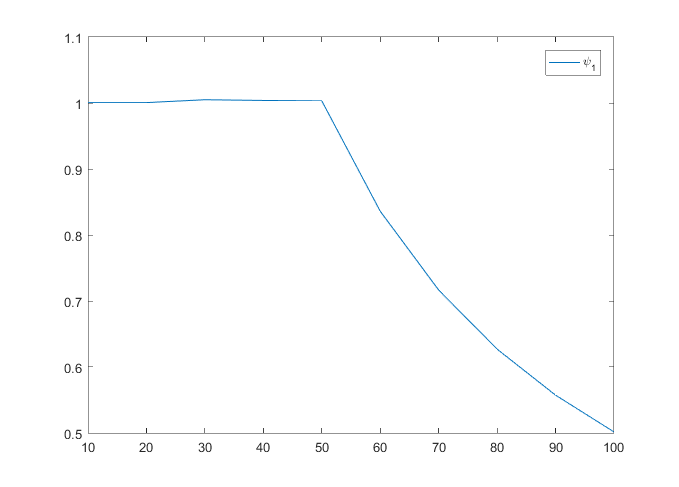
\includegraphics[width = \textwidth]{./Bilder/f_psi}
	\caption{Betrag der Statorflussverkettung $\psi_1$}
	\label{fig:Statorflussverkettung}
\end{figure}
%
\begin{figure}[htb]
	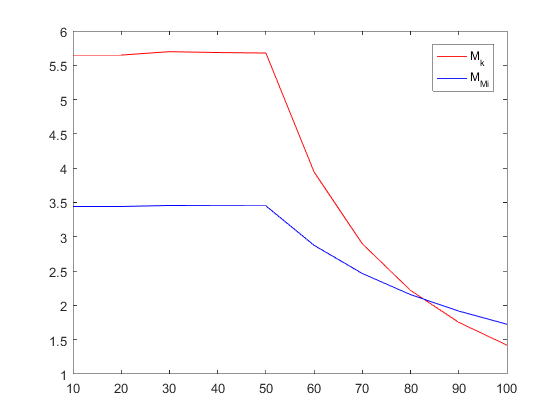
\includegraphics[width = \textwidth]{./Bilder/f_moment}
	\caption{Verlauf Kippmoment $M_k$ und Motormoment $M_Mi$}
	\label{fig:momente}
\end{figure}
\newpage
\section{}\label{sec:aufg6c}
%
Das Motormoment $M_Mi$ wird folgendermaßen berechnet und ist in Abb. \ref{fig:momente} dargestellt.
\begin{equation}
M_Mi = \frac{3}{2}\cdot Z_P \cdot \frac{\textit{\^{U}}}{\omega} \cdot \textit{\^{I}} \cdot cos(0.7)
\end{equation}